\documentclass[12pt]{revtex4-1}

\usepackage{graphicx} % needed for figures
\graphicspath{ {Figures/} }
\usepackage{epstopdf}
\usepackage[caption=false]{subfig}
\usepackage{amsmath}
\usepackage{amsfonts}
\usepackage{amssymb}
\usepackage{bm}
\usepackage{hyperref}
\usepackage{amsthm}
\usepackage{color}
\newcommand{\DB}[1]{\textcolor{cyan}{#1}}
\usepackage{mathrsfs}
\usepackage[vlined,ruled]{algorithm2e}
%\usepackage{subfigure}
%\usepackage{cite}
\usepackage{url}
\usepackage{color}
\usepackage{algorithmic}
\usepackage{bbm}
\usepackage{booktabs}
\usepackage{array}
\usepackage[table]{xcolor}
\usepackage{yfonts}

\newtheorem{theorem}{Theorem}[section]
\newtheorem{lemma}[theorem]{Lemma}
\newtheorem{definition}{Definition}
\newtheorem{corollary}[theorem]{Corollary}
\newtheorem{proposition}[theorem]{Proposition}
\newtheorem{problem}{Problem}
\newtheorem{remark}{Remark}
\newtheorem{assumption}{Assumption}
\newtheorem{example}{Example}

\newcommand{\mc}{\mathcal}
\newcommand{\Ker}{\operatorname{Ker}}
\newcommand{\Rank}{\operatorname{Rank}}
\newcommand{\Image}{\operatorname{Im}}
\newcommand{\real}{\mathbb{R}}
\newcommand{\complex}{\mathbb{C}}
\newcommand{\ora}[1]{\overrightarrow{#1}}
\newcommand{\map}[3]{#1: #2 \rightarrow #3}
\newcommand{\subscr}[2]{{#1}_{\textup{#2}}}
\newcommand{\supscr}[2]{{#1}^{\textup{#2}}}

\begin{document}
\title{Design of Mechanical Motions with Discrete Dynamical Systems}
\date{\today}
\begin{abstract}
	The function of many mechanical systems often depends on conformational changes in structure. To achieve desired functions, we must first accomplish the design of desired conformational changes. Here, we model mechanical systems as linkages of rigid bonds (edges) connected by joints (nodes), and map this design problem to the theory of discrete dynamical systems. Specifically, we begin by showing that a small linkage module can be thought of as one dimensional map of node distances. Next, we demonstrate that combining these modules together is equivalent to an iteration of this map. Finally, we demonstrate the design power of this map by constructing mechanical networks that display fixed points, limit cycles, and aperiodicity.
\end{abstract}
\maketitle

\section{Mathematical Framework}
\subsection{Mechanical Networks}
Consider a set of $N$ nodes $\mc V = \{1, \dotsm, N\}$ connected by $E$ pairwise edges $\mc E \subset \mc V \times \mc V$ in $d$-dimensional space. Each node $i$ has a real vector of coordinates $\bm{x}_i \in \real^d$, and the edge $k$ between nodes $i,j$ has squared length given by
\begin{align*}
l_k^2 = (\bm{x}_i - \bm{x}_j)^T(\bm{x}_i - \bm{x}_j).
\end{align*}
To enforce rigid edges, we take the time derivative of the length, and set $\dot{l}_k = 0$ such that
\begin{align*}
2l_k\dot{l}_k = 2(\bm{x}_i-\bm{x}_j)^T(\dot{\bm{x}}_i-\dot{\bm{x}}_j) = 0
\end{align*}
We can concatenate all node coordinates into column vector $\bm{x} = [\bm{x}_1; \dotsm; \bm{x}_N] \in \real^{dN}$, and all edge measurements into column vector $\bm{l} = [l_1^2; \dotsm; l_k^2]$. Then the coordinates yield $dN$ free variables, while the rigid edges yield $E$ constraints given by $\dot{\bm{l}} = \bm{0}$ such that we have $dN - E$ possible motions by constraint counting. Among these, $d(d+1)/2$ are rigid body translations and rotations, for $D$ conformational motions given by
\begin{align*}
D = dN - E - \frac{d(d+1)}{2}.
\end{align*}

\subsection{Dynamical Systems}
Additionally, consider a one-dimensional discrete-time dynamical system with state variable $r_n \in \real$ at some time $n \in \mathbb{Z}_{\geq 0}$ that evolves according to
\begin{align*}
r_{n+1} = f(r_n). 
\end{align*}
This iterated map exists in a $k$-cycle if
\begin{align*}
r_{n+k} = f^k(r_n),
\end{align*}
where $f^k$ implies the application of the map $k$-times. This $k$-cycle is stable if the product of slopes evaluated along the cycle $r_{n+1},\dotsm,r_{n+k}$
\begin{align*}
s = \prod_{i=1}^k \frac{d}{dr}f(r)\bigg|_{r_{n+i}},
\end{align*}
has magnitude less than $|s| < 1$. 




\section{Mechanical Modules as a Discrete-Time Map}
Consider a network with $D = 1$ conformational motion such as the 4-bar linkage shown in Figure~\ref{fig:4bar} (left). Here, we have $N=4$ nodes, $E = 4$ edges for $D = 8-4-3 = 1$ conformational motion, and this motion manifests as a smooth, one dimensional change in network conformation (Fig.~\ref{fig:4bar} center). We can assign the distance one pair of unconnected nodes as $r_1$ (Fig.~\ref{fig:4bar} red), and another pair as $r_2$ (Fig.~\ref{fig:4bar} blue), and plot $r_2$ as a function of $r_1$ along this continuous conformational motion (Fig.~\ref{fig:4bar} right). If we take $r_n$ to be our discrete-time state variable, then this plot defines a function such that $r_2 = f(r_1)$. 

\begin{figure}[h!]
	\centering
	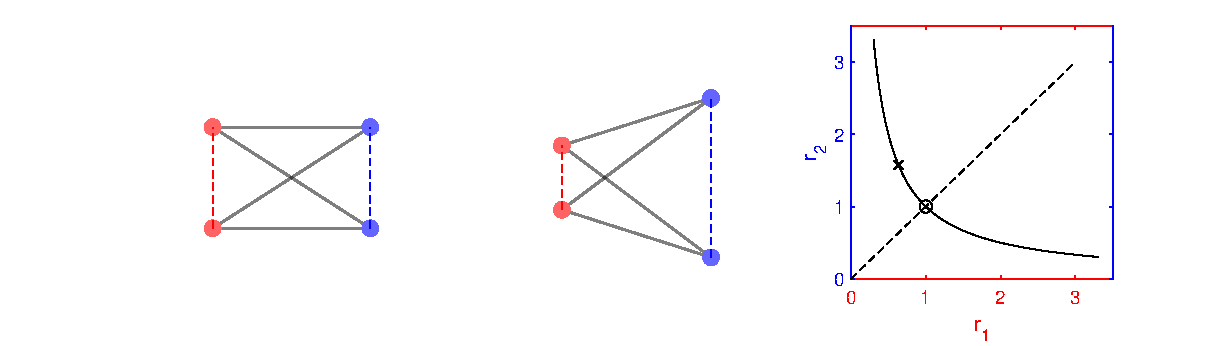
\includegraphics[width=1.0\columnwidth]{4bar.pdf}
	\caption{\textbf{Network Module as Discrete-Time Map.} \textbf{(Left):} Simple 4-bar linkage with nodes as circles, edges as gray lines, and the distance between red nodes as dashed red line $r_1$, and blue nodes as dashed blue line $r_2$. \textbf{(Center):} Same linkage undergoing continuous conformational change. \textbf{(Right):} Plot of $r_2 = f(r_1)$ as a function of $r_1$, with the original configuration marked with a circle, and the deformed configuration with an X, with the line $r2 = r1$ as a dashed line.}
	\label{fig:4bar}
\end{figure}



\section{Map Iteration Through Module Combination}
Next, consider two of these modules (Fig.~ \ref{fig:combined} top-left), where each module has distance $r_1$ and $r_2$. If we combine these modules by overlapping the nodes as indicated by the dashed line, then we merge our node distances such that $r_2$ of the left module becomes $r_1$ of the right module. The combined network now has three distances: $r_1$ (red), $r_2$ (magenta), and $r_3$ (blue) (Fig.~\ref{fig:combined} bottom-left), such that $r_2 = f(r_1)$, $r_3 = f(r_2)$, and $r_3 = f(f(r_1))$. Hence, chaining networks such that $r_1$ of the new module connects to $r_2$ of the old module yields an iterated map that can be analyzed using methods such as cobweb plots (Fig.~\ref{fig:combined} right).

\begin{figure}[h!]
	\centering
	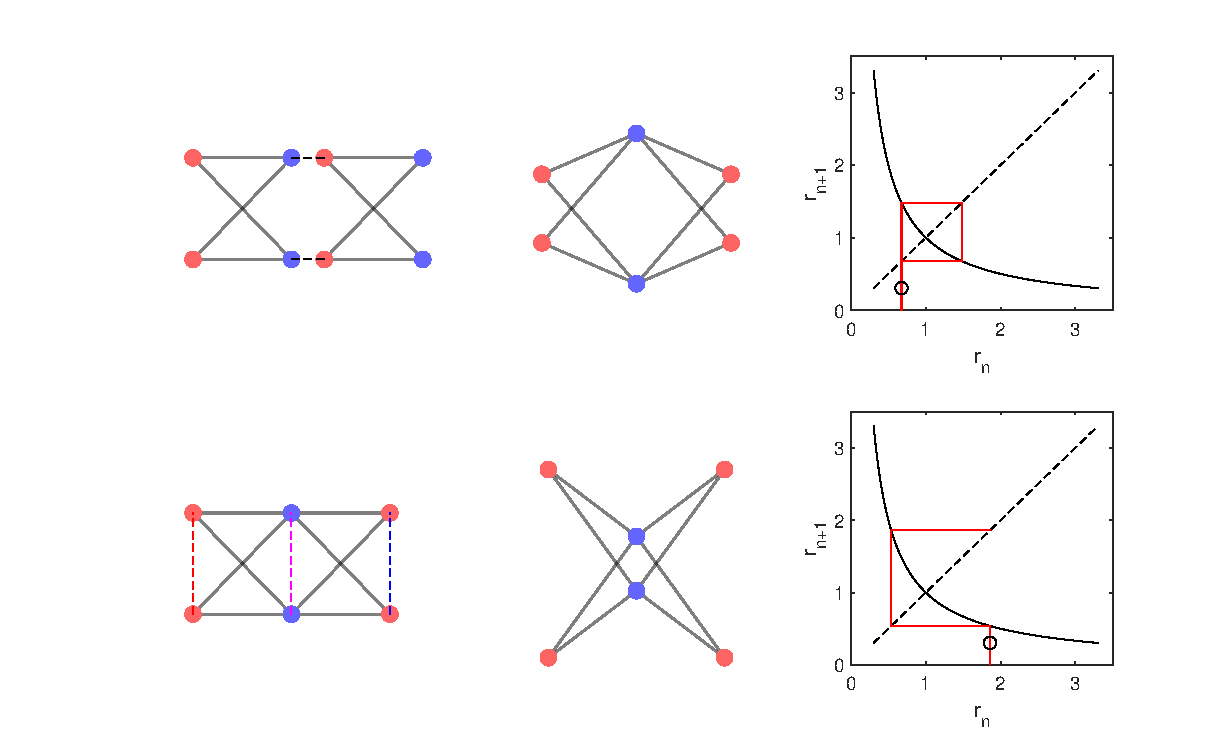
\includegraphics[width=1.0\columnwidth]{combined.pdf}
	\caption{\textbf{Map Iteration through Module Combination.} \textbf{(Top-Left):} Two identical 4-bar linkages, where the nodes to be combined are connected by dashed lines. \textbf{(Bottom-Left):} The combined linkage of 6 nodes, 8 edges, with $r_1$ as red, $r_2$ as magenta, and $r_3$ as blue. \textbf{(Top-Center):} Contracted, and \textbf{(Bottom-Center):} expanded forms of the networks. \textbf{(Top-Right):} Cobweb plot of $r_1, r_2, r_3$ of the contracted, and \textbf{(Bottom-Right):} expanded forms.}
	\label{fig:combined}
\end{figure}



\section{Network Design with Nonlinear Dynamics}
In our previous work "Conformational Control of Mechanical Networks," we outlined principles for designing finite and infinitesimal conformational changes. These principles amount to designing the function $r_{n+1} = f(r_n)$ by picking two points along $f$, as well as the slope $dr_{n+1}/dr_n$ at one of these points. 

\subsection{Super-Stable Fixed Point}
In this context, a fixed point is simply a repeating network module in the same conformational state. Using the bipartite principles from the past paper, we specify the positions and instantaneous motions of the first part (Fig.~\ref{fig:fixed_point} top-left), and compute the solution space satisfying distance constraints for the second part (solid blue line), where the distance between the nodes of the first part are $r_1$ (green) and $r_2$ (cyan). Then, we construct the network by placing the second part nodes (blue) and edges until $D=1$ (Fig.~\ref{fig:fixed_point} top-center), and we plot $r_2$ \emph{versus} $r_1$ along this conformational trajectory to confirm that 1) our initial configuration exists at a fixed-point, and 2) the slope of $r_2 = f(r_1)$ is 0 (Fig.~\ref{fig:fixed_point} top-right). As before, we can iterate this map by coupling the $r_2$ nodes of one module to the $r_1$ nodes of an identical module (Fig.~\ref{fig:fixed_point} bottom). 


\begin{figure}[h!]
	\centering
	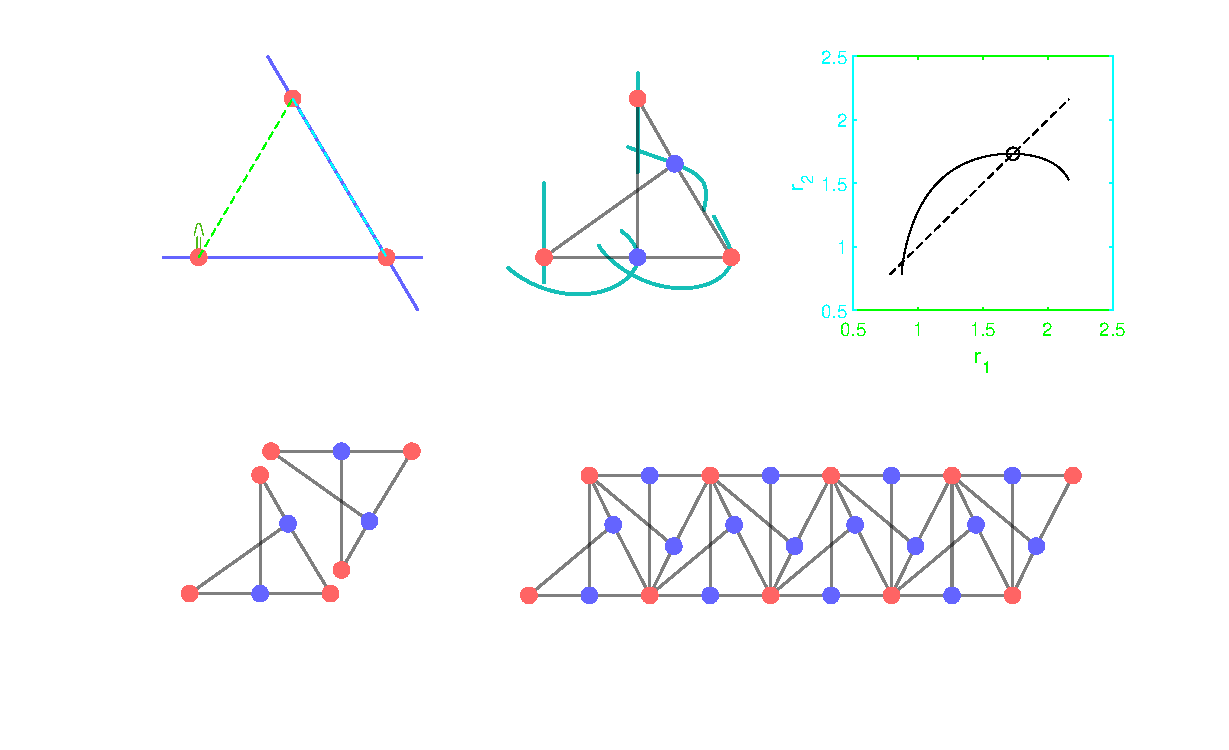
\includegraphics[width=1.0\columnwidth]{fixed_point.pdf}
	\caption{\textbf{Construction of Super-Stable Fixed Point.} \textbf{(Top-Left):} Specified node positions (red) and motions (green arrow), with distance $r_1$ as the dashed green line, and $r_2$ as the dashed cyan line. \textbf{(Top-Center):} Trajectory (green lines) of the constructed network with $D=1$. \textbf{(Top-Right):} Corresponding plot of trajectory for $r_2 = f(r_1)$, where the circle represents the originally designed configuration. \textbf{(Bottm-Left):} Coupling two identical modules by combining the nearest pair of red nodes. \textbf{(Bottom-Right):} Large coupled network.}
	\label{fig:fixed_point}
\end{figure}

Intuitively, the distance between the left-most nodes corresponding to the original $r_1$ act as initial conditions for the remainder of our network. However, we see that because the fixed point is super-stable, our system should maintain the fixed-point configuration under massive perturbation to initial condition. This is indeed what we see in Figure.~\ref{fig:fixed_point_sim}, where the $D=1$ conformational motion sequentially collapses the network from the left along a collapsing front, where the network is rigid both to the left and right of the collapsing front.

\begin{figure}[h!]
	\centering
	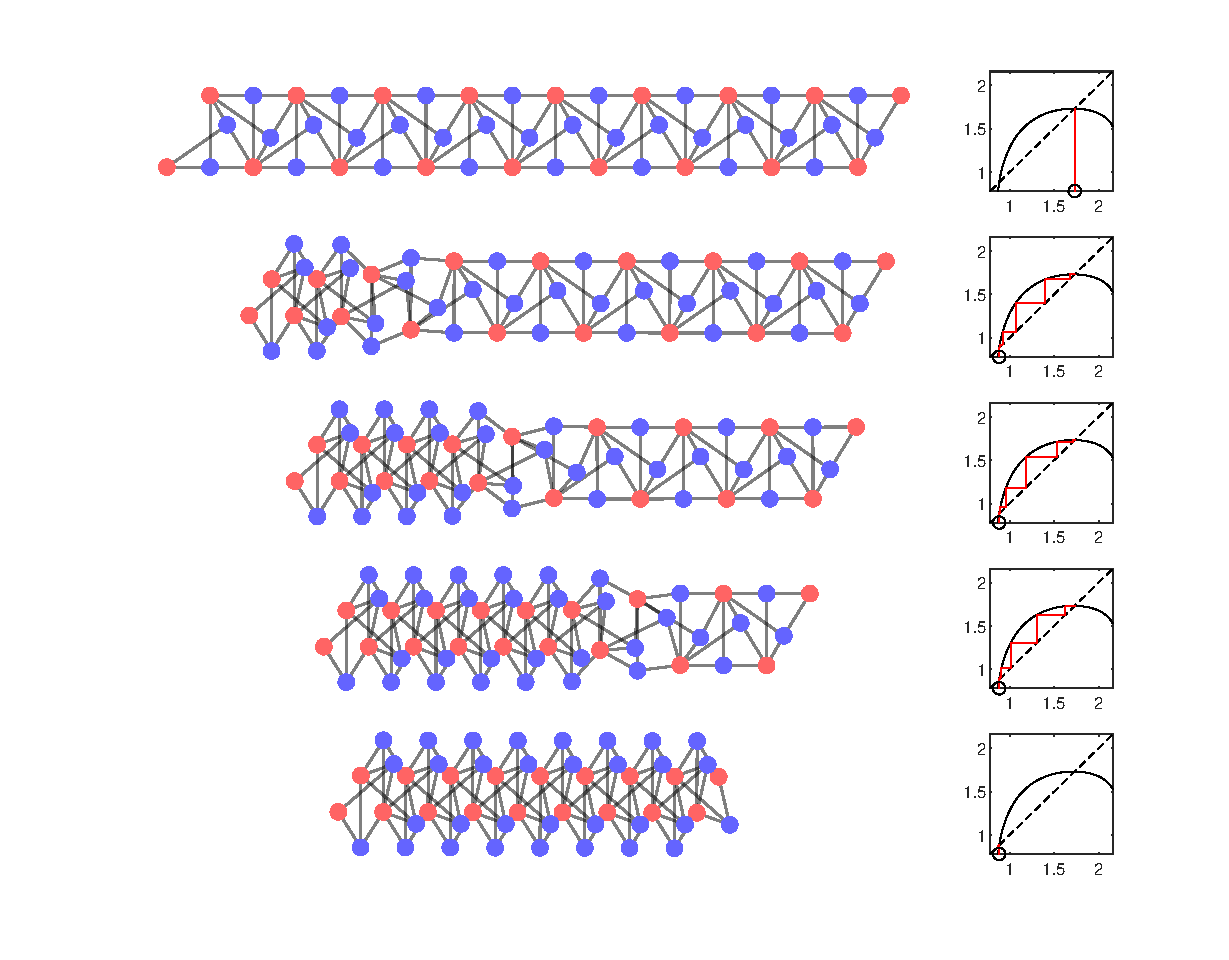
\includegraphics[width=1.0\columnwidth]{fixed_point_sim.pdf}
	\caption{\textbf{Simulation of Super-Stable Fixed Point.} \textbf{(Left):} Simulation of combined network along $D=1$ conformational motion. \textbf{(Right):} Cobweb plot along the iterated map with varying initial conditions shown as a circle.}
	\label{fig:fixed_point_sim}
\end{figure}

\subsection{Aperiodic Map}
The natural subsequent question is whether we can construct a chaotic/aperiodic map. We construct such a network that has the shape of a tent-map (Fig.~\ref{fig:aperiod}). Here, the fixed point is unstable, as is the limit cycle. Further, the function is closed in that for any $r_n$ shown on the curve, the range of the function $r_{n+1} = f(r_n)$ remains fully within the domain. 

\begin{figure}[h!]
	\centering
	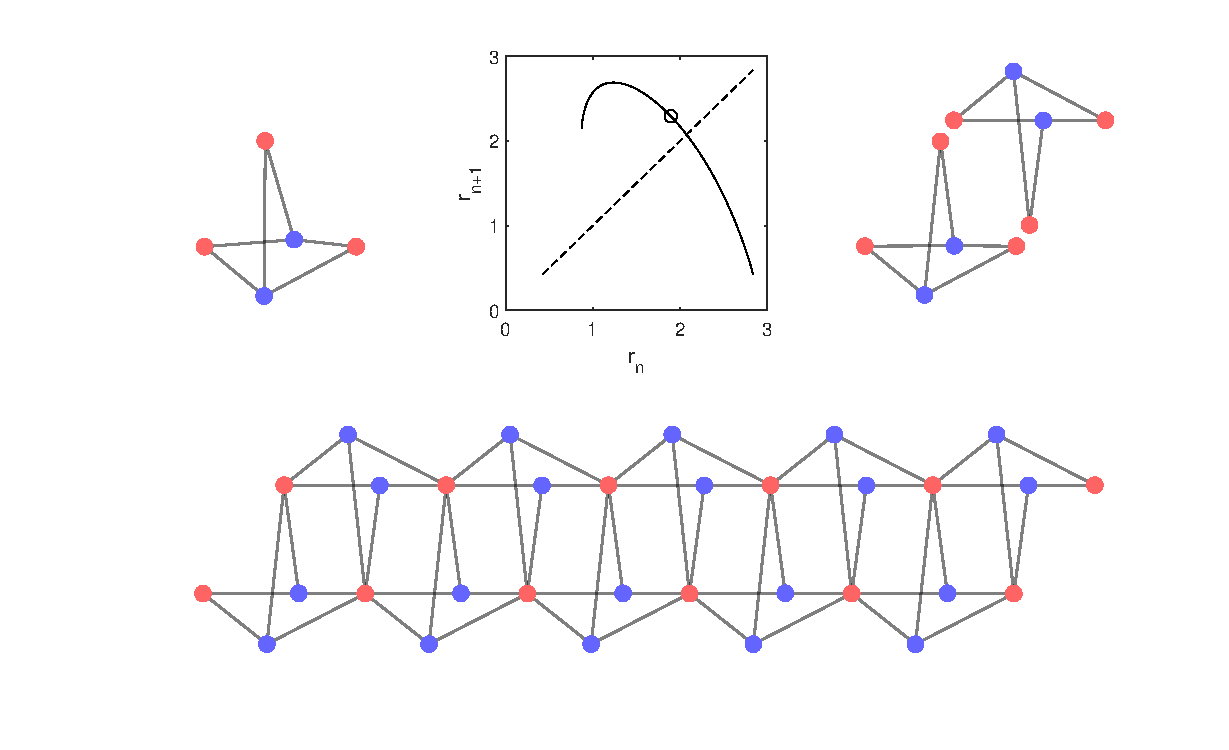
\includegraphics[width=1.0\columnwidth]{aperiod.pdf}
	\caption{\textbf{Construction of Aperiodic Network.} \textbf{(Top-Left):} Construction of aperiodic network with \textbf{(Top-Center):} corresponding iterated map, coupled together according to \textbf{(Top-Right)} to generate large network \textbf{(Bottom)}.}
	\label{fig:aperiod}
\end{figure}

We show the $D=1$ conformational motion by slowly stretching $r_1$, the distance between the left-most nodes, along with the corresponding cobweb plots in Figures~\ref{fig:aperiod_sim}, \ref{fig:aperiod_sim2}. Note that at the fixed point, the structure remains there in the crystal state. However, small deviations in the initial condition yield complex and dramatic shifts in the remainder of the network. 

\begin{figure}[h!]
	\centering
	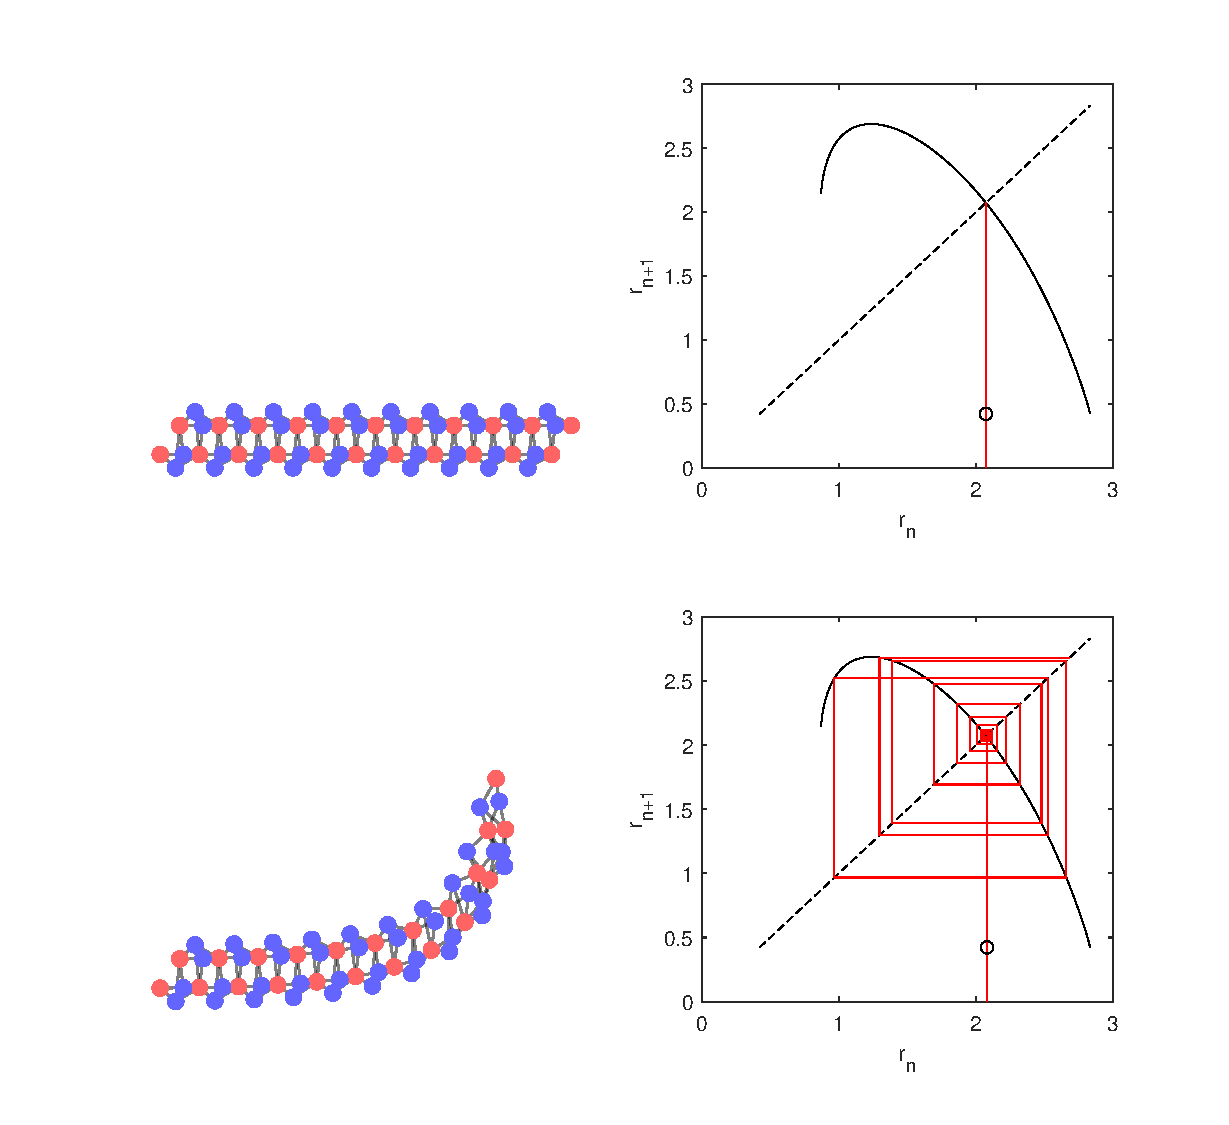
\includegraphics[width=1.0\columnwidth]{aperiod_sim.pdf}
	\caption{\textbf{Aperiodic Network.} \textbf{(Left):} Same networks starting at different initial conditions (distances $r_1$ between the left-most red nodes), with \textbf{(Right):} corresponding cobweb plot.}
	\label{fig:aperiod_sim}
\end{figure}

\begin{figure}[h!]
	\centering
	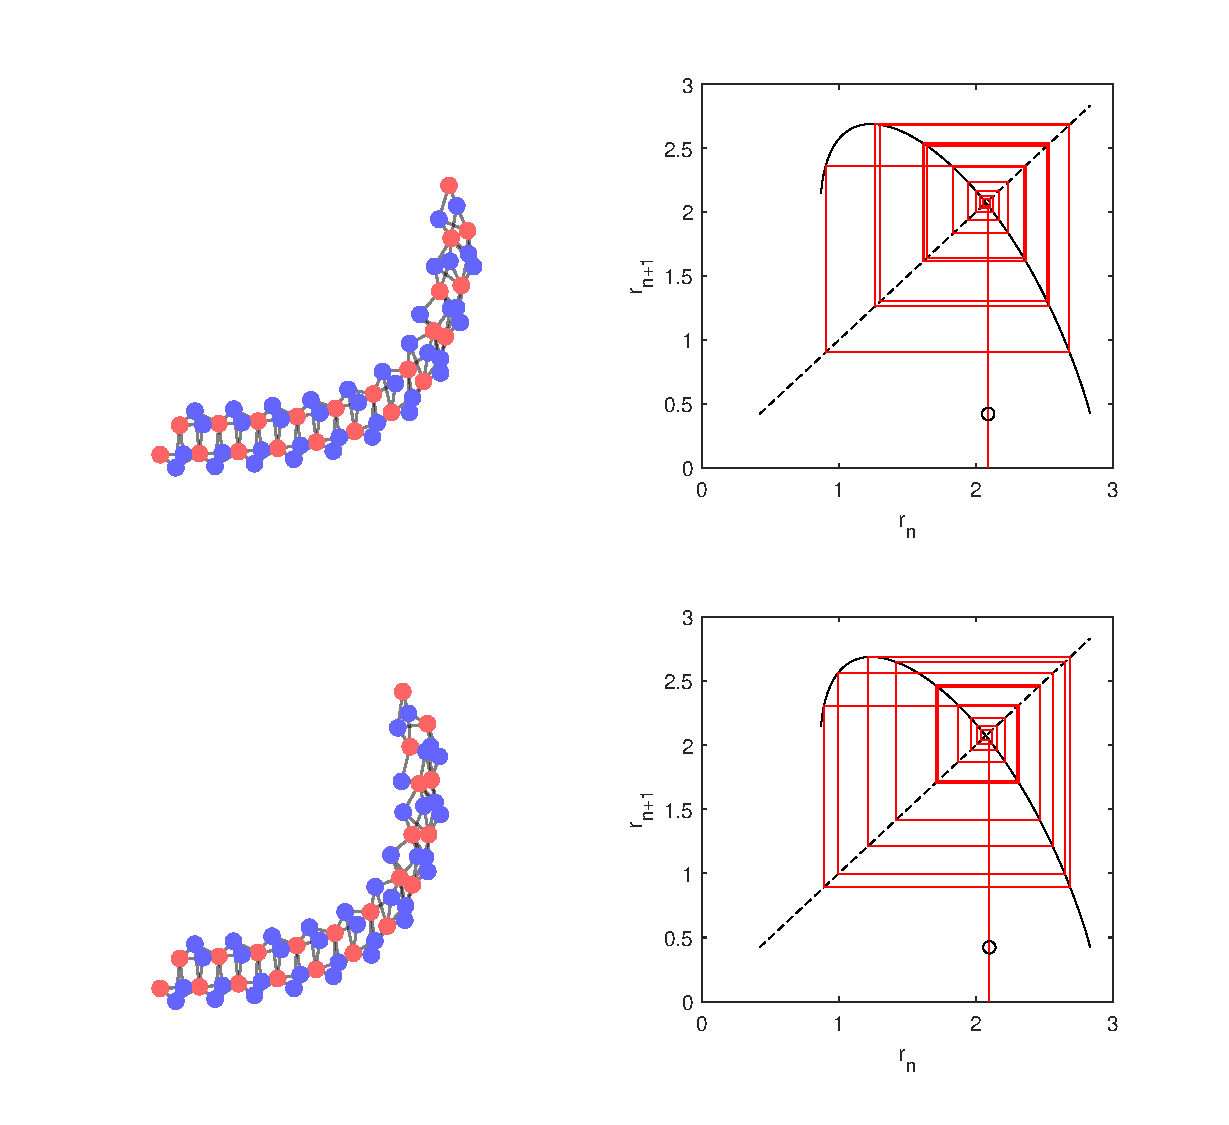
\includegraphics[width=1.0\columnwidth]{aperiod_sim2.pdf}
	\caption{\textbf{Aperiodic Network.} \textbf{(Left):} Same networks starting at different initial conditions (distances $r_1$ between the left-most red nodes), with \textbf{(Right):} corresponding cobweb plot.}
	\label{fig:aperiod_sim2}
\end{figure}



\end{document}
